\documentclass[../../norme-di-progetto.tex]{subfiles}

\begin{document}

\subsubsection{Finalità}%
\label{subs:accertamento_della_qualita/finalita}

GruppOne istanzia il processo di accertamento della qualità per garantire qualità di processo e di prodotto.
Gli esiti dei processi di verifica e validazione saranno indispensabili nello svolgimento del processo di accertamento della qualità.

\subsubsection{Descrizione}%
\label{subs:accertamento_della_qualita/descrizione}

Il processo di accertamento della qualità garantisce che i prodotti e i processi del ciclo di vita del software rispettino i requisiti prestabiliti e che aderiscano ai piani esecutivi prefissati.
Gli obiettivi e le strategie che il team si impegna ad applicare durante lo svolgimento del progetto sono presentati nel \textit{Piano di qualifica (versione \versione)}.

\subsubsection{Attività}%
\label{subs:accertamento_della_qualita/attivita}

Le principali attività coinvolte nel processo di accertamento della qualità sono:

\begin{itemize}
  \item Accertamento della qualità di prodotto
  \item Accertamento della qualità di processo
  \item Accertamento del sistema di qualità.
\end{itemize}

\paragraph{Accertamento della qualità di prodotto}%
\label{par:accertamento_della_qualita_di_prodotto/attivita}
L'attività di accertamento della qualità di prodotto assicura la qualità dei processi di fornitura del prodotto e promuove controlli continui, che possano garantire i requisiti e le funzionalità concordate, e prevenire il verificarsi di danni non recuperabili.
È fortemente dipendente dalla qualità di processo: da processi privi di qualità, infatti, non è possibile ottenere buoni prodotti.

Il riferimento principale che adottiamo per questo asse di qualità è lo standard ISO/IEC 25010:2011, ponendo particolare attenzione alle caratteristiche che hanno maggiore interesse per il proponente del prodotto.

\paragraph{Accertamento della qualità di processo}%
\label{par:accertamento_della_qualita_di_processo/attivita}

L'attività di accertamento della qualità di processo monitora i processi istanziati, e deve essere perseguita nel corso del ciclo di vita del software in modo che il prodotto soddisfi le richieste del proponente e che i processi convergano con costi ridotti in termini di risorse a pari qualità di prodotto.
Per avere un sistema efficace di accertamento della qualità di processo è necessario che il team:

\begin{itemize}
  \item Individui i processi da controllare.
  \item Stabilisca le metriche di valutazione del processo.
  \item Esegua accertamenti continui sui processi scelti.
  \item In base ai risultati ottenuti, ricerchi un miglioramento continuo dei processi.
\end{itemize}

Per questo asse di qualità lo standard principale che adottiamo è ISO/IEC 90003:2014, pur considerando che per la natura del progetto la sua applicazione avrà portata limitata allo svolgimento del progetto stesso.

\paragraph{Accertamento del sistema di qualità}%
\label{par:accertamento_del_sistema_di_qualita}

L'attività di accertamento del sistema di qualità è strettamente legata allo standard ISO 9001:2005.
Per svolgerla, Gruppone adotta come modello il ciclo PDCA, o ciclo di Deming, un metodo di gestione dei processi che permette di attuare un continuo miglioramento dei processi stessi.

\subsubsection{Procedure}%
\label{subs:accertamento_della_qualita/procedure}

\paragraph{Ciclo di Deming}%
\label{par:ciclo_di_deming}

Il ciclo di Deming è un metodo applicabile a tutti i processi istanziati da GruppOne che sfrutta la ripetizione di quattro attività:

\begin{description}
  \item [Plan] definisce gli obiettivi, le attività e i processi necessari per raggiungere i risultati attesi.
  \item [Do] esegue ciò che è stato definito nella fase di pianificazione.
  \item [Check] verifica gli esiti dei processi.
  \item [Act] esegue azioni correttive per migliorare la qualità dei processi.
\end{description}

\begin{figure}[H]
  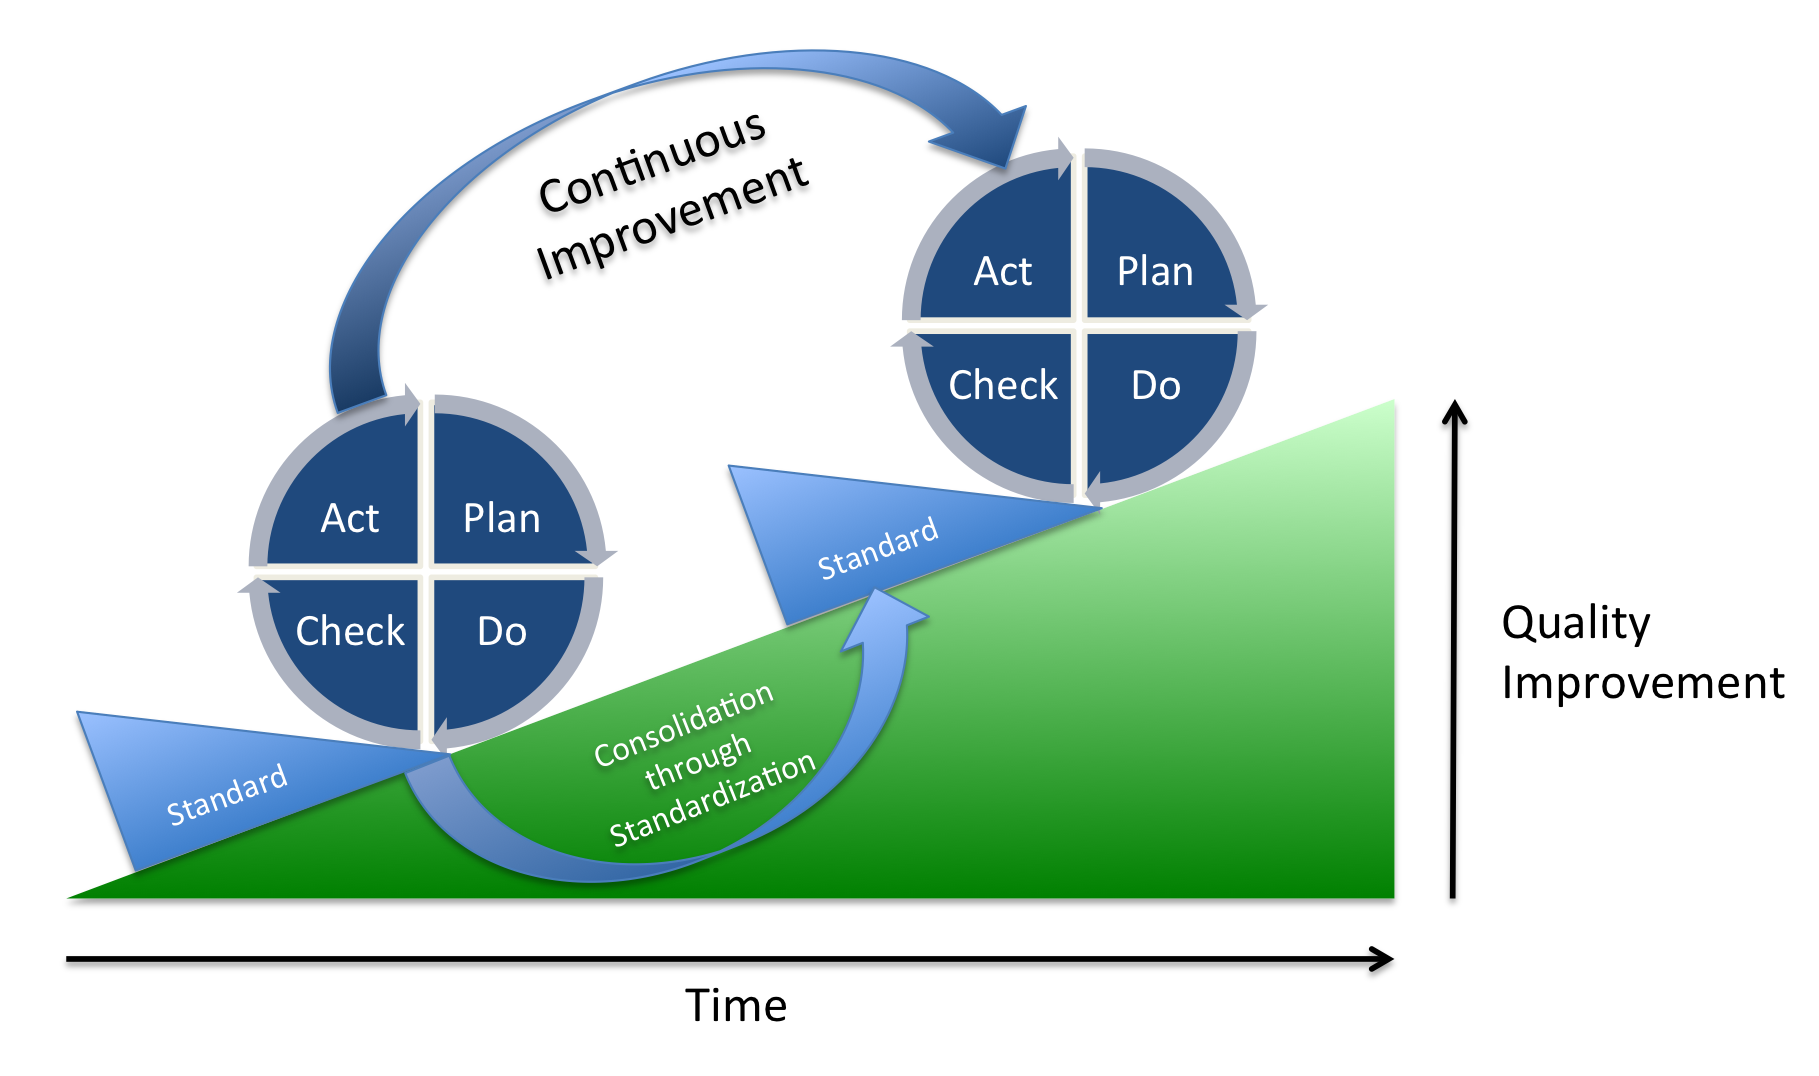
\includegraphics[width=8cm]{PDCA-process.png}
  \centering
  \caption{ciclo di Deming o PDCA.}
\end{figure}

\subsubsection{Metriche}%
\label{subs:accertamento_della_qualita/metriche}

\paragraph{Denominazione delle metriche}%
\label{par:denominazione_delle_metriche}

Le metriche sono essenziali per avere una misura oggettiva di qualità del nostro prodotto, e vengono definite durante la pianificazione del processo di accertamento della qualità.
Per tale ragione per la definizione delle metriche di qualità è necessario identificare una denominazione comune.
Ogni metrica avrà la seguente struttura:
\begin{center}
  \textbf{M[Tipo][Sigla]}
\end{center}
\begin{description}
  \item [Tipo] indica il tipo di metrica. Può essere:
        \begin{description}
          \item[PS]: metrica di processo
          \item[PR]: metrica di prodotto
          \item[TS]: metrica di test.
        \end{description}
  \item [Sigla] indica una sigla che abbrevia la metrica.
\end{description}

\paragraph{Percentuale delle metriche soddisfatte in maniera eccellente (MPS-PME)}%
\label{par:percentuale_delle_metriche_soddisfatte_in_maniera_eccellente}

La metrica permette di conoscere la percentuale delle metriche soddisfatte in maniera eccellente rispetto a tutte le metriche  disponibili.
La formula della metrica è la seguente:
\[
  PME = \frac{MSOD}{MTOT} \times 100
\]
dove:
\begin{description}
  \item[PME] risultato che indica la percentuale di metriche.
  \item[MSOD] numero di metriche soddisfatte, dove per \textit{soddisfatte} si intende tutte le metriche che hanno superato una certa soglia di accettabilità.
  \item[MTOT] numero totale di metriche.
\end{description}

Ecco una lista che indica che significato assume PME\@:
\begin{itemize}
  \item Se il risultato è pari a 0\%, nessuna metrica è stata superata.
  \item Se il risultato è pari al 100\%, tutte le metriche sono state soddisfatte.
  \item Se il risultato è maggiore di 0\%, ma minore di 100\%, non tutte le metriche sono state soddisfatte.
\end{itemize}

%\subsubsection{Procedure}%
%\label{subs:accertamento_della_qualita/procedure}

%\subsubsection{Strumenti di supporto}%
%\label{subs:accertamento_della_qualita/strumenti_di_supporto}

\end{document}
